\documentclass{beamer}




\usetheme{Copenhagen}

\author{Jos\'{e} A. Mu\~{n}iz Navarro} 
\title{A Comparison of Algorithms for Building ST-Histograms} 
\institute{MIT} 

\begin{document}

	\begin{frame}
		\maketitle	
	\end{frame}
	
	
\begin{frame}
  \tableofcontents
\end{frame}

	%
	%Slide 1:
	% How do we use histograms in database systems?
	%
	
	
	\begin{frame}
		\section{Motivation}
		\frametitle{Histograms help database systems optimization}�
			\begin{itemize}
				\item Tables have fields
				\item One histogram per field. 
				\item Selectivity helpful for optimizing queries
			\end{itemize}
			
		
		\begin{columns}[C]
		

  			\begin{column}{0.4\textwidth}
				\bigskip
				
				Need to sort by age
				
				\begin{itemize}
					\item Insertion sort?
					\item Merge sort?
				\end{itemize}
			\end{column}



  			\begin{column}{0.4\textwidth}
    				\begin{center}
					 \includegraphics[width=90pt]{TableStudents.PNG} 
				\end{center} 
			\end{column}
			

			
		\end{columns}�
		
	\end{frame}	



	\begin{frame}
			\frametitle{How to calculate selectivities from histograms}

    				\begin{center}
					\texttt{FIND students WITH AGE� age $\leq 14 $ }

					  \only<1>{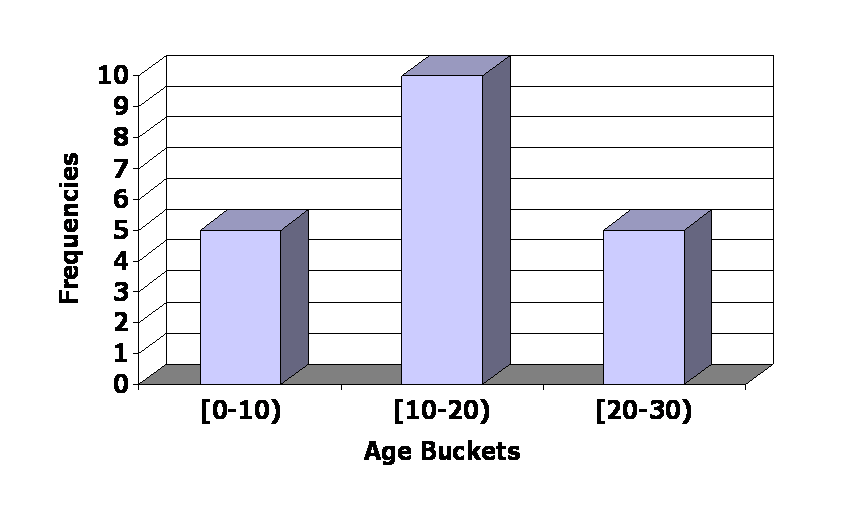
\includegraphics[width=130pt]{RegHistogram.PNG}}
					  \only<2>{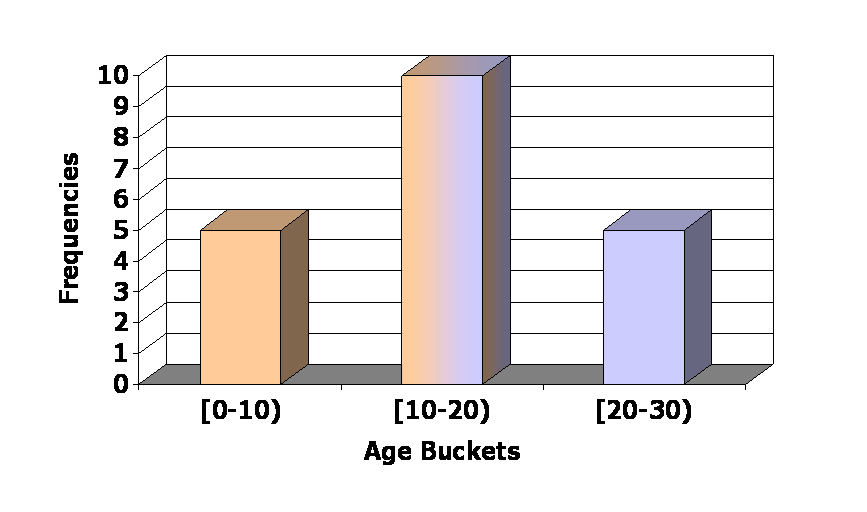
\includegraphics[width=130pt]{RegHistogramSel.PNG}}
				\end{center}

		\bigskip
				
	\only<2> {�$$\sigma =  5 + \frac{10}{2} = 10 $$} 

	\end{frame}
		
	
	
	%
	%Slide 2:
	% How do we build histograms?
	%
	\begin{frame}
		\section{Previous Work}

		  \frametitle{Building histograms: Traditional cost-based optimization}
		
		\begin{columns}[T]
  			\begin{column}{0.3\textwidth}
    				Four components: 
    				\begin{itemize}
				      \item Optimizer
				      \item Executor
				      \item Histogram
				      \item Statistics gatherer
				\end{itemize}
		   	\end{column}

			 \begin{column}{0.7\textwidth}	
				 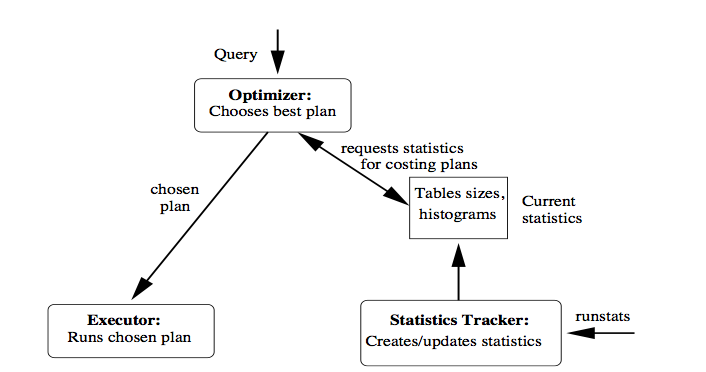
\includegraphics[width=200pt]{TraditionalPlan.PNG} 

			 \end{column}
		\end{columns}

			\bigskip
			
			No connection between executor and histogram. 
			

			
	\end{frame}	

	
	%Slide 3: 
	% Problems with model
	\begin{frame}
	
		\frametitle{Some problems with traditional approach}�	

			
			Problems: 
			
			\bigskip 
			
			\begin{itemize}
				\item Tradeoffs
					\begin{itemize}
						\item performance $\leftrightarrow$ adaptability
						\item performance $\leftrightarrow$ precision
				\end{itemize}				
				\item Postgres suggests turning off statistics analyzer for large tables!
				
			\end{itemize}			
		
	\end{frame}


	%Slide 4: 
	% Solution : ST-Histograms
	\begin{frame}
	
		\frametitle{Idea: Incremental build via Self Tuning Histograms}�	
			
			Previous work by
			\begin{itemize}
				\item Aboulnaga and Chaudhuri - ST Histograms
				\item Babu, Bizarro - Adaptive Query Processing
				
			\end{itemize}
			
					
				\bigskip 
				
				 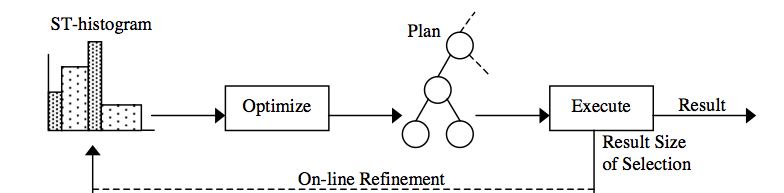
\includegraphics[width=300pt]{STModel.PNG} 
			
		\pause 
		{Interface}
				\begin{itemize}
				\item Executor executes \\
					~~\texttt{emit([a...b], val)}
				\item Histogram builder provides \\
					~~\texttt{int estimate([a...b])}
				\end{itemize}
			
	
	\end{frame}


	%Slide 5: 
	% Some details
	\begin{frame}
	
		\frametitle{Self Tuning Histograms: Interface and Motivation}�	

		\begin{itemize}
			\item {How do we build the histogram without looking at data?}
				\begin{itemize}
					\item Update frequencies
					\item Update buckets
				\end{itemize}
				
		\end{itemize}

	\end{frame}


	\begin{frame}
	
		\frametitle{Updating frequencies}�	

			Result from \texttt{emit([0,19], 30)}
			
			 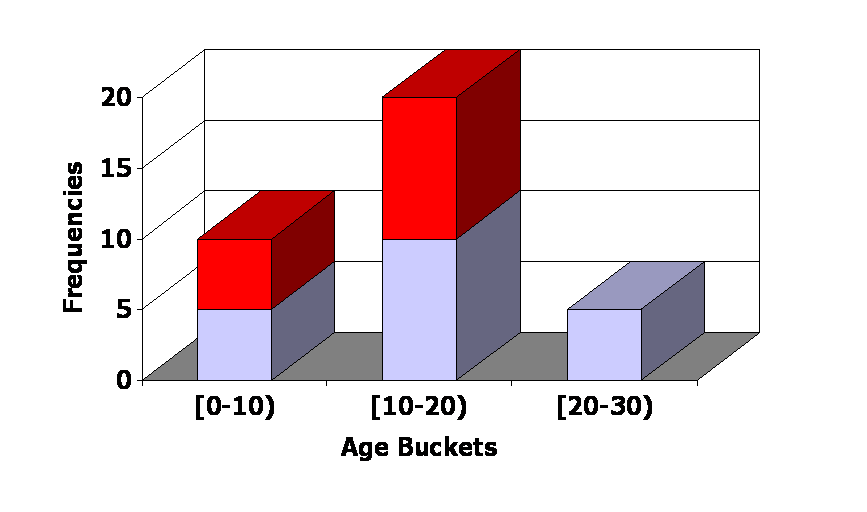
\includegraphics[width=300pt]{emit0-19-30.PNG} 

				
	\end{frame}
	


	\begin{frame}
	
		\frametitle{Merge and split}�	

			
			 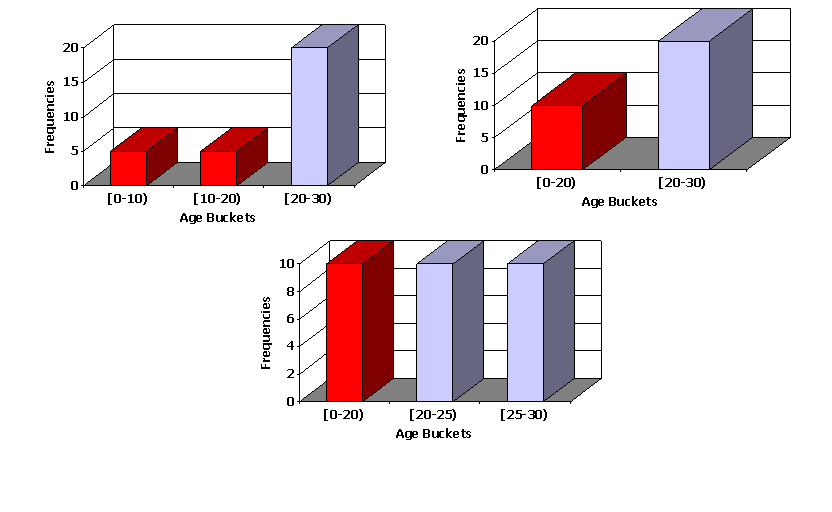
\includegraphics[width=300pt]{merge-split.PNG} 

				
	\end{frame}
	



	%Slide 6: 
	% Algorithm I
	\begin{frame}
		\section{Proposal}
		
		
		
		\frametitle{Proposed work}�	

		\begin{center}
		Determine feasibility of implementing ST Histograms in transactional databases, 
		by benchmarking different ST algorithms against a common database system. 
		\end{center}

		\bigskip
		Algorithm modifications: 
		\begin{itemize}
			\item Occasionally renormalize data to fit to total number of tuples.\\
				\emph{Improves determination of error vs insertion}
			\item Adjust blame proportional to range and frequency
			\item Split most frequently updated ranges
		\end{itemize}
				
	\end{frame}
	
	
	
		
	
	
	%Slide 6:
	%Experimental Setup
	\begin{frame}
	
		\frametitle{Proposed Setup}�	

		
		\begin{itemize}
			\item Middle layer between database and end user
			\item Process: 
				\begin{enumerate}
					\item Relay query to database
					\item Obtain query plan from database
					\item Simulate query, using results for calling \texttt{emit}
					\item Calculate error rate in generated histograms
				\end{enumerate}
			
			\item Measure performance gains over common statistics gathering in  
				transactional loads. 
				
		
		\end{itemize}

				 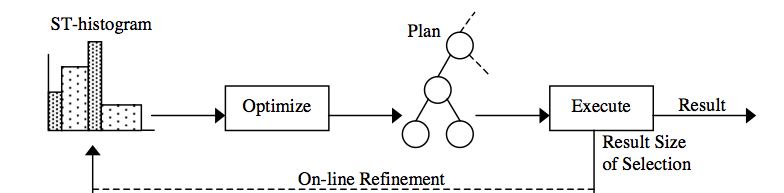
\includegraphics[width=300pt]{STModel.PNG} 


	 \end{frame}
	
	%Slide 8:
	%Timeline
	\begin{frame}
	
		\frametitle{Expected Results}�	
		
		\begin{itemize}
			\item Fast to adapt 
			\item Minimal insertion overhead (Small amount of tuples per query)			
				\begin{itemize}
					\item Ideal for large databases with constant insertions
						and varying ranges. 
				\end{itemize}
		\end{itemize}

		\bigskip

		Caveats: 
		\begin{itemize}
			\item Major optimizer misses due to independence assumptions,
				and not failures in row estimates. 
			\item Not all cases lead to performance gains. 
			\item No solution for \texttt{LIKE} queries.  
			 
		\end{itemize}
				

		
	\end{frame}
	
	
	\begin{frame}
		\begin{itemize}
			\item Week 1: Build parser
			\item Week 2: Build executor
			\item Week 3: Build histogram builder
			\item Week 4-5: Implement different histogram building algorithms
			\item Week 6-7: Implement TPC-C benchmark
			\item Week 8-10: Run statistics and gather data
			
		\end{itemize}
	\end{frame}
	

	
 
\end{document}